\input{/Users/jovo/Research/latex/latex_paper.tex} 
\usepackage{url}
\lhead{Vogelstein JT, et al}
\rhead{short title}

\newcommand{\mcE}{\mathcal{E}}
\newcommand{\mcT}{\mathcal{T}}
\newcommand{\mcG}{\mathcal{G}}
\newcommand{\mcM}{\mathcal{M}}
\newcommand{\mcL}{\mathcal{L}}
\newcommand{\hatmcE}{\widehat{\mcE}}
\newcommand{\hatp}{\widehat{p}}
\newcommand{\hatP}{\widehat{P}}
\newcommand{\hatQ}{\widehat{Q}}
\newcommand{\hatL}{\widehat{L}}
\newcommand{\mhP}{\widehat{\PP}}
\newcommand{\tildeA}{\widetilde{A}}
\newcommand{\GG}{\mathbb{G}}

\newcommand{\defa}{\begin{defi}}
\newcommand{\defb}{\end{defi}}

\newtheorem{Rem}{Remark}%[section]
\newtheorem{Alg}{Algorithm}%[section]
\newtheorem{Thm}{Theorem}[section]
%\theoremstyle{marginbreak}
\newtheorem{Lem}{Lemma}[section]
%\newtheorem{Lem}[Cor]{Lemma}
%\theoremstyle{change}
%\theorembodyfont{\itshape}
\newtheorem{Def}{Definition}[section]

\title{PRE-DRAFT: On unlabeled graph classification}

\author{jv1,jv2,djm,jmc,cep}
% JV1 ; Henry ; \dots

\begin{document}

\maketitle
% \tableofcontents



\begin{abstract}
	
Many kinds of data are better characterized by graphs than vectors, including social networks, telecommunication grids, and brains.  It is often desirable to compare two or more of these graphs with one another.  Unfortunately, sometimes these graphs are unlabeled, meaning there is no known correspondence between vertices on one graph and vertices on another graph. In such scenarios, making comparisons is relatively difficult, as it typically first requires at least approximately solving the ``graph matching'' or ``graph isomorphism'' problem.  

% although two general strategies are possible.  First, one can compute a number of ``graph invariants,'' that is, scalar measures of graphs that are invariant to vertex permutations.  Second, one can solve the graph isomorphism problem (GIP), effectively aligned graphs with one another, as close as can be aligned.  
Because no known algorithm can solve GIP in polynomial time, one is often forced to use approximate solutions.  We provide several approximations to GIP, and show how performance scales with computational time.  We compare various approaches, using somewhat idealized simulations, as well as simulations based on real brain-graph data, and finally real human brain-graph data.

\end{abstract}

\section{Introduction}

In the current digital age, swaths of data are collected in myriad diverse fields ranging from astronomy to zoology.  While these data are well characterized by networks, or graphs, the vast majority of statistical inference techniques, including the recent advances in machine learning, tend to assume the data live in finite dimensional Euclidean space.  Thus, inference techniques designed to specifically to address collections of graphs could potentially yield fruitful results across many domains.  Furthermore, these collections of graphs often lack vertex labels, meaning the function labeling each vertex in each graph is unknown.  In such scenarios, the graphs are called ``unlabeled,'' and this is the scenario of interest for this manuscript.  Consider, for example, two food networks in different jungles.  Both might have lions and tigers and bears (oh my), so it is easy to compare across the jungles.  On the contrary, if one jungle only has the birds and the bees, one might still be interested in comparing the food networks, but a bird might play the same role in the second jungle as the lion does in the first, making comparisons across jungles more complicated.


The exploitation task of investigation for this manuscript is that of unlabeled graph classification.  More specifically, we assume that we have observed some number of unlabeled graph/class pairs, and we want to classify a novel unlabeled graph into its appropriate class. Unfortunately, because we do not directly observe the complete graphs, rather, only the unlabeled version of each graph, our classifiers must somehow deal with this additional complication.

We consider two general approaches.  First, one can compute a large number of statistics on unlabeled graphs that are invariant to isomorphisms.  That is, if $g$ is a graph, and $\mt{g}$ is another graph isomorphic to $g$, then any function that satisfies $f(g)=f(\mt{g})$ is called a ``graph invariant.''  For example, the number of edges or triangles in a graph is invariant to isomorphisms.  By computing a large number of these graph invariants, one effectively projects the graph into finite Euclidean space, at which time one can apply standard machine learning tools.  A second approach under consideration involves first (approximately) solving the graph matching (also known as the graph isomorphism) problem (GIP) for each test graph, and then applying \emph{labeled} graph classification algorithms, such as those developed in \cite{VogelsteinPriebe10a}.

Neither of these approaches are likely to dominate the other in general, as both have rather severe limitations.  The graph invariant approach lacks much rigorous theoretical support.  For instance, it remains an open question for which distributions can the graph invariant approach achieve the Bayes optimal classification rate (except in trivial cases for which the generative model is a function of the particular graph invariants being used). However, many graph invariants can be computed quite quickly.  Further, graph invariants have both local and global properties, that is, they capture some aspect of the whole graph, by recursively considering local functions.  Finally, for certain exploitation tasks, one might desire to understand the relationship between certain graph invariants and the class (for instance, are transportation grids more efficient when more triangles exist?).  

On the other hand, if one first (approximately) solves GIP, then limiting results for many classifiers are readily available (upon representing each graph as an adjacency matrix that resides in finite  Euclidean space).  Unfortunately, solving GIP is known to be NP incomplete \cite{??} (not known to be NP complete nor P).   This means that solving GIP remains quite computationally expensive, especially as $n$, the number of vertices in the graphs, gets large.

Several questions therefore arise for us, as a first investigation into unlabeled graph classification.  Are there distributions for which approximate GIP solutions yield good classification results? If so, can we establish any general rules under which approximating GIP is expected to perform relatively well?  Alternately, are there distributions for which the graph invariant approach outperforms the GIP approach?  How do the computations and performances for these two approaches scale with respect to one another?  In this study, we first describe precisely how one might proceed upon using either of the above two approaches.  Then, we conduct a number of in simulu experiments that we believe are informative with regard to some of these questions.  We conclude with some discussion and outlines for possible future work and applications.

\section{Methods} % (fold)
\label{sec:methods}

\subsection{Preliminaries} % (fold)
\label{sub:nomenclature}

% subsection nomenclature (end)

Let $G$ be a graph-valued random variable, $G: \Omega \mapsto \mc{G}$, where $\mc{G}$ is the set of all possible graphs, $g \in \mc{G}$ (and $\Omega$ is the universal sample space). A graph is assumed to be a triple, $(V,A,Q)$, where $V=\{V_i\}=V_i \, \forall i \in [n]=\{1,\ldots,n\}$ is the set of vertices, $A=\{A_{ij}\}$ is the adjacency matrix, each edge is binary (an easily relaxed assumption), and $Q$ is a permutation matrix (a matrix with a single one in each column and row, and zeros otherwise). Let $\mc{A}=\{0,1\}^{n \times n}$ be the space of all possible adjacency matrices, and $\mc{Q}$ denote the set of permutation matrices.

Further, let $Y$---the \emph{class} of an object---be a binary-valued random variable, $Y: \Omega \mapsto \mc{Y} = \{0,1\}$, which can be easily generalized to any multinomial space (or continuous spaces with a bit more work).  Graphs and classes are sampled jointly and exchangeably from some unknown but true distribution, $\PP_{\bth}[G,Y] \in \mc{P}$, where $\mc{P}$ is the family of distributions under consideration, $\mc{P} = \{\PP_{\bth}[G,Y] : \bth \in \Theta\}$, $\bth$ is the parameter of the distribution, and $\Theta$ is the set of all possible parameters (in the sequel, we often drop the $\bth$ from $\PP_{\bth}[G,Y]$).  

Formally, we assume that  $(G,Y), \{(G_s,Y_s)\} \sim \PP_{\bth}[G,Y]$, where $(G,Y)$ is the graph/class test sample pair, and $\mc{T}_S=\{G_s,Y_s\}=\{(G_1,Y_1),\ldots, (G_S,Y_S)\}$ is the training sample set, where $S$ is the total number of training samples.  The goal is to impute the latent test sample class, $Y=y$, given the training data.  While we do not believe that $\PP_{\bth}[G,Y]$ is in fact true for any possibly extant data, we do believe that the true distribution (if one exists) can be approximated reasonably well by some distributions in $\mc{P}$, such that we have hope to achieve misclassification rates better than chance on at least some data sets.  

Unfortunately, we do not observe the graphs in their entirety, but rather, the permutation matrices are latent (we will often implicitly assume that vertices are observed).  That is, instead of observing $G_s=(A_s,Q_s)$, we observe only $A_s$.  Throughout, we will use the notation that $\mt{A}_s = Q_s A_s Q_s\T$, so, had we observed $\mt{A}_s$'s, then we would have observed all there is to perform the classification.  Note that graph invariants can therefore be defined as functions on $A$, that is if $f(A,Q)=f(A)$ for all $A\in \mc{A}$ and all $Q \in \mc{Q}$, then $f(\cdot)$ computes a graph invariant.


\subsection{Optimal approach} % (fold)
\label{sec:lik}

The Bayes optimal classifier is:
\begin{align}
	\mh{y} = \argmax_{y \in \{0,1\}} \PP[G,Y] = \argmax_{y \in \{0,1\}} \PP[G | Y] \PP[Y]
\end{align}
where $\PP[G|Y]$ is the \emph{likelihood} of observing a graph given its class, and $\PP[Y]$ is the prior probability of each class.  By obtaining estimates of these two terms, one can build a plugin classifier:
\begin{align}
	\mh{y} = \argmax_{y \in \{0,1\}} \mhP[G | Y] \mhP[Y]	
\end{align}
where $\mhP[G|Y]$ and $\mhP[Y]$ are the plugin estimates of the likelihood and prior, respectively.  Estimating the prior is trivial, one can simply use the maximum likelihood estimator, $\mh{\pi}=\mhP[Y=1]$ and $1-\mh{\pi}=\mhP[Y=0]$.  The likelihood term, however, is more complex.  It can be expanded:
\begin{align}
	\PP[G|Y] = \PP[A,Q | Y] = \PP[A | Y] \PP[Q]
\end{align}
as the adjacency matrix, $A$, and permutation matrix $Q$, are conditionally independent given the class label, $Y$.  Further, the permutation matrix is assumed to be independent of the class label.  Thus, if $Q$ were observed, then estimating $\PP[A|Y]$ would be all there is to it; unfortunately, $Q$ is latent, and thus must be imputed for each example.  

To proceed, we define an explicit likelihood model, which we will use in the sequel.  Because each element of the adjacency matrix is binary, edges are Bernoulli random variables.  We assume that each edge is independent, but not identical.  If the permutation matrix was known to be the identity matrix, we would have:
\begin{align}
\PP[A,Q|Y] = \prod_{ij} \text{Bernoulli}(a_{ij}; \eta_{ij}^y)
\end{align}
However, because the permutation matrix is in general, not the identity, we instead have:
% , yielding the following model:
% The likelihood of a new graph, $G=(A,Q)$ is therefore a prod defined as follows: %. For the adjacency matrix, we assume here the independent edge model, that is:
\begin{align}
\PP[A,Q|Y] = \prod_{ij} \text{Bernoulli}\bigg(\sum_{ij} q_{ij} q_{ji} a_{ij}; \eta_{ij}^y\bigg) \PP[Q]
% \eta_{ij}^{\sum_{ij} q_{ij} q_{ji} a_{ij}}
 % \prod_{ij} \PP[A_{ij}, Q | Y]	= \prod_{ij} \text{Bernoulli}(a_{ij}; \eta_{ij}^y) = \prod_{ij} \big(\eta_{ij}^y\big)^{a_{ij}'}\big(1-\eta_{ij}^y\big)^{1-a_{ij}'}.
\end{align}
The permutation matrix has the following distribution:
\begin{align}
	\PP[Q] = \sum_{Q \in \mc{Q}} \delta_Q w_{Q}
\end{align}
where $\delta_Q$ is an indicator function taking unity value whenever $Q'=Q$ and zero otherwise, and $w_Q$ is the likelihood of any particular permutation matrix, where $w_Q\leq 0$ and $\sum_{Q}w_Q'=1$.  The simplest assumption is that each permutation matrix is equally likely, that is: $w_Q'=1/n!$, because $n!$ is the number of $n\times n$ element permutation matrices.  

The log-likelihood of $\PP[A,Q|Y]$, ignoring the $\PP[Q]$ term is:
\begin{align}
	\mc{L}(\mb{\eta},Q)  = \sum_{ij} \bigg\{\Big[\sum_{ij} q_{ij} q_{ji} a_{ij} \ln \eta_{ij}\Big] + \Big[ \Big(1+\sum_{ij} q_{ij} q_{ji} a_{ij}\Big) \ln (1-\eta_{ij})\Big]\bigg\}
\end{align}
The goal is then to maximize the log-likelihood with respect to both $\mb{\eta}$ and $Q$:
\begin{align}
	(\mh{\eta},\mh{Q}) = \argmax_{\mb{\eta} \in (0,1)^{n\times n} ,Q \in \mc{Q}} \mc{L}(\mb{\eta},Q),
\end{align}
which is difficult in part due to the constraint on $Q$.  But one can relax that constraint to allow $Q$ to be any doubly-stochastic matrix, which is a natural relaxation, given that permutation matrices are the extreme points of the set of doubly stochastic matrices.  A matrix is said to be doubly stochastic if both all the rows and all the columns sum to unity.  Thus, to maximize the log-likelihood, we have:
\begin{align}
	(\mh{\eta},\mh{Q}) \approx \argmax_{\eta \in  (0,1)^{n\times n}, Q \in \mc{D}} \mc{L}(\mb{\eta},Q),
\end{align}
where $\mc{D}$ is the set of doubly stochastic matrices.  Using Lagrange multipliers, we can rewrite \label{eq:mle}:
\begin{align}
	(\mh{\eta},\mh{Q}) \approx \argmax_{\eta \in  (0,1)^{n\times n}} \mc{L}(\mb{\eta},Q) - \lambda (1 - \tfrac{1}{n}\mb{1}\T Q) - \lambda (1 - \tfrac{1}{n}\mb{1}\T Q\T),
\end{align}
where the additional terms impose the constraint that the columns and rows sum to one, respectively.  Now, the likelihood term is concave in $\eta$ (but not $Q$), and the constraints are linear, and therefore concave in $Q$, thus, one can use a coordinate ascend strategy, optimizing $Q$ followed by optimizing $\eta$, until convergence. This ignores the $Q$ terms in the likelihood.  Perhaps somebody (else) could figure out how to (at least approximately) account for those.  Regardless, this is an approximate solution to finding the most likely permutation matrix for each sample, as well as the independent edge probabilities.   


\subsection{Quadratic assignment problem approximation} % (fold)
\label{sub:graph_isomorphism_approach}


Instead of the likelihood based approach outlined above, one could consider the permutation matrices ``nuisance parameters,'' and construct \emph{some} way to estimate them, and plug that value in, assuming it is ``correct.'' Note that the disadvantage of this approach relative to the likelihood based approach is that it is less ``natural'' from a statistical point of view, for example, modeling averaging is not quite as obvious, and incorporating prior information might also be less obvious.  The advantage, however, is that much work as already been devoted to solving closely related problems,  and we can therefore piggyback on the shoulders of giants.  %In this case, we piggyback on the shoulders of Marguerite Frank and Phil Wolfe, who developed the Frank-Wolfe (FW) algorithm for solving quadratic programming problems with linear constraints.  

More specifically, assume we have the same model assumed above in Section \ref{sec:lik}, and assume that $\eta$ is known, such that we must only estimate the permutation matrix.  This problem is closely related to the graph matching (or graph isomorphism) problem (GIP), in which, given any pair of graphs, one searches for the permutation matrix that makes them as similar as possible.  ``Similarity'' can be defined as desired, with some definitions perhaps better than others in some domains.  The likelihood is one measure of similarity, and since the classifier that we are using is a likelihood based classifier, the likelihood is the ``best'' measure of similarity for this problem.  However, since we cannot solve the likelihood approach, instead, we look for a measure of similarity as close to likelihood as possible.  Least squares seems like a reasonable guess, given the close relationship between least squares, maximum likelihood estimation, and Kullback-Leibler divergence \cite{YangPriebe10, Grunwald07} (although absolute distance is another reasonable approach, and efficient algorithms exist \cite{}):  
\begin{align} \label{eq:qap}
	\mh{Q} &= \argmin_{Q \in \mc{Q}} \norm{Q A Q\T - B}^2_F
\end{align}
where $A$ and $B$ are two arbitrary adjacency matrices, $\norm{\cdot}_{F}$ indicates the Froebenius norm, $\norm{x}_F=\sum_{ij} \sqrt{x_{ij}^2}$.  Unfortunately, because the set of permutation matrices, $\mc{Q}$, is discrete, optimizing over them is difficult.  Eq. \eqref{eq:qap} is closely related to a well studied problem, called the \emph{quadratic assignment problem}.  Noting that $Q\T Q=I$, where $I$ is the identity matrix, is true for any orthogonal $Q$, and that permutation matrices are orthogonal, Eq. \eqref{eq:qap} can be rewritten:
\begin{align} \label{eq:qap}
	\mh{Q} &= \argmin_{Q \in \mc{Q}} \norm{Q A Q\T - B}^2_F
			\\ &= \argmin_{Q \in \mc{Q}}tr\big((QAQ\T-B)\T(QAQ\T-B)\big)
			\\ &= \argmin_{Q \in \mc{Q}}tr(QA\T Q\T QA Q\T)  - tr(B\T QAQ\T) - tr(QAQ\T B) + tr(B\T B)
			\\ &= \argmin_{Q \in \mc{Q}}tr(QA\T A Q\T)  - tr(B\T QAQ\T) - tr(QAQ\T B)
			\\ &= \argmin_{Q \in \mc{Q}} - tr(B\T QAQ\T) - tr(QAQ\T B),			
\end{align}
which is equivalent to the standard representation of the quadratic assignment problem \cite{}:
\begin{align}
	\mh{\sigma}= \argmin_{\sigma} a_{\sigma(i), \sigma(j)} b_{ij} = \argmin_{q \in \mc{Q}} q_{ij} a_{ij} q_{ji} b_{ij}
\end{align}
where $\sigma$ is a permutation, that is, $\sigma: [n] \mapsto [n]$, and the second equality follows from the definition of a permutation matrix.  

In fact, solving GIP is known to be $NP$ incomplete (meaning it is not known to be in either $P$ or $NP$) \cite{??}.  Therefore, instead of trying to solve this exactly, we make approximations to make it easier.  


 % Pseudocode for the FW algorithm to approximately solve the QAP is provided below:
% \begin{Alg}[Frank-Wolfe Algorithm (FW)]
% Given $ Q^{(1)} \in \mathcal D_m $.
% %\roster \widestnumber\item{xxxxxxxx} \raggedright
% \item {Step 0:} Let $k$ = 1.
% 
% \item {Step 1:} Let $\nabla_Q^{(k)} = A Q^{(k-1)} B\T + A\T Q^{(k-1)} B$.  
% 
% \item {Step 2:} Compute $W^{(k)}$  by solving the
% linear assignment problem:
% % $$
% \begin{align}
% 	W^{(k)} = \argmin_{W^{(k)} \in \mc{D}} %{\text{\rm arg }} \min_{W^{(k)}}
% 	% \lbrace { 
% 	\sum_{i,j=1}^m 
% 	\left( 
% 	\nabla_Q^{(k)}\circ W^{(k)}
% 	 \right)_{ij}
% 	% }\rbrace	
% \end{align}
% % $$
% % \item {Step 3:} Let $d^{(k)} = W^{(k)} - Q^{(k-1)}. $
% \item {Step 3:} Find $\alpha^{(k)} \in [0,1]$ such that
% $$\alpha^{(k)}=\argmin_{\alpha^{(k)}}
% \mc{L} (Q^{(k)} + \alpha^{(k)} W^{(k)}).
% $$
% \item {Step 4:} Let
% 
% $$ Q^{(k+1)} = Q^{(k)} + \alpha^{(k)} W^{(k)}. $$
% \item {Step 5:} 
% If $\norm d^{(k)}_{P} \norm \le \epsilon$ or $\alpha^{(k)}=0$ or $k=k_{\max}$
% then stop; else $k$ = $k$ + 1 and go to step 1.
% \end{Alg}
\subsection{Graph invariant based classifiers (it is not obvious to me that it is even worth comparing the graph invariant classification, as this study is really about performance degradation when $Q$ is unknown, and the utility of additional iterations)} % (fold)
\label{sub:graph_invariant_based_classifiers}

Many graph invariants are available from the literature (see 
\url{http://en.wikipedia.org/wiki/Graph_invariant}
for a list of some of the most popular ones).   A subfield of random graph models, collectively called exponential family random graph models (ERGMs), typically models a graph by its triangles, $k$-stars, and the like \cite{??}.  Recent work from Pao et al. analyzed the power of various graph invariants for a special case of hypothesis testing \cite{??}.  Because of the close relationship between hypothesis testing and classification (see B\&D, pg. XXX \cite{??}), we consider the same set of graph invariants here.  In particular, we consider:
\begin{enumerate}
	\item size:  $\#(A)$ = the number of edges in the graph
	\item  maximum degree: $\del(G)= \max_{i \in [n]} d(V_i)$, where $d(V_i)$ indicates degree of vertex $i$, that is, the number of edges incident to $V_i$.
	\item maximum average degree: 	$MAD(G)=\max_{\Omega_G} \bar{d}(\Omega_G)$, where $\bar{d}(G)$ is the average degree of a graph, and $\Omega_G$ is all subgraphs of $G$.  Because computing $MAD(G)$ exactly is computationally taxing (how much???), we instead compute the maximum eigenvalue $MAD$ \cite{PaoPriebe10}.
	\item scan statistics: the $k$-th scan statistic is the maximum number of edges over all $k$-th order neighborhoods, $S_k(G) = \max_{i \in [n]} \#(\Omega_{N_k[i;G]})$, where $N_k[i;G]=\{j \in [n] : l(V_i,V_j) \leq k\}$, and $l(V_i,V_j)$ is the distance between any two vertices, that is, the minimum number of edges traversals between them.  We assume that $l(V_i,V_i)=0 \, \forall i$, and $l(V_i,V_j)=\infty$ if no path exists between $V_i$ and $V_j$.
	\item number of triangles:  a triangle exists whenever there is an edge from $V_i$ to $V_j$, one from $V_j$ to $V_k$, and one from $V_k$ back to $V_i$
	\item clustering coefficient: a measure that captures the degree to which nodes tend to cluster together
	\item average path length: typically defined by $\sum_{i,j} l(V_i,V_j)/(n^2-n)$, but to exclude the infinities, we let $\infty \mapsto 2 \max l(V_i,V_j)$.
\end{enumerate}

Let $\mb{f}(\cdot): \mc{G} \mapsto \Real^k$ be the function that takes a graph as input, and outputs a set of $k$ graph invariants.  Having defined such a function, one can then use standard machine learning algorithms to perform classification.  We plug the results into a ``standard'' suite of machine learning tools: (i) a linear classifier---linear discriminant analysis (LDA), (ii) a quadratic classifier---quadratic discriminant analysis (QDA), (iii) a support vector machine (SVM), (iv) random forests (RF), and (v) $k_n$ nearest neighbor classifier.  Note that the dimensionality of the data is quite large ($\mc{O}(n^2)$), we first reduce the dimensionality of the data using principal components analysis (PCA).  The dimensionality of the data to keep is chosen using the method of \cite{??}.



\subsection{Simulations} % (fold)
\label{sub:simulations}

In all the below simulations, as mentioned above, we assume the data is sampled exchangeably, that is: $(G,Y), \{(G_s,Y_s)\} \overset{exch.}{\sim} \PP[G,Y; \eta]$, where $G=(V,A,Q)$.  Further, we assume an independent edge model
\begin{align}
\PP[A,Q | Y] &= \PP[A|Q,Y] \PP[Q] = \prod_{i,j \in [n]} \text{Bernoulli}\left(\sum_{ij} q_{ij} q_{ji} a_{ij}; \eta_{ij}^y\right) \sum_{Q\in \mc{Q}} \delta_Q/n! \\
&=  \prod_{i,j \in [n]} \text{Bernoulli}\left(\mt{a}_{ij}; \eta_{ij}^y\right) \sum_{Q\in \mc{Q}} \delta_Q/n!
\end{align}
where $\mt{a}_{ij} = \sum_{ij} q_{ij} q_{ji} a_{ij}$.  This means that the class-conditional distributions are just the matrices $\eta^0$ and $\eta^1$, where $\eta^y=\{\eta_{ij}^y\}$. Moreover, the class-conditional difference is therefore also a matrix, $\delta=\{\delta_{ij}\}$, where
\begin{align}
	\delta_{ij} = | \eta_{ij}^1-\eta_{ij}^0|.
\end{align}
We also define the relative class-conditional differences
\begin{align}
	\delta_{ij}^r = \left| \frac{\eta_{ij}^1}{\eta_{ij}^1 (1-\eta_{ij}^1)} - \frac{\eta_{ij}^0}{\eta_{ij}^0 (1-\eta_{ij}^0)} \right|
\end{align}
which normalizes differences by their magnitude, similar to z-scores for comparing Gaussian distributed random variables. For each of the below simulated experiments, we generated $S=100$ training samples, half from each class, and two test samples, one from each class.  






% paragraph homogeneous_kidney_egg_simulation (end)






% subsection simulations (end)

\section{Results} % (fold)
\label{sec:results}

% section results (end)

\subsection{General QAP Test Problems}
%\label{sec:genqap}
%\begin{enumerate}
%\item  QAPLIB - Burkard, Karisch, Rendl [1994] \cite{burkard:1994}
%\item  $n$: 5 - 128
%\end{enumerate}
To illustrate the effectiveness of FW 
we give the performance of the algorithm on 16 sample problems.  The below table gives the optimum value found by FW with 1, 2, 3, and 100 random starting points   and compared 
to the best known solution as given in column 2 and the Path algorithm  \cite{Path:2009}, column 7.   The starting point for FW, $X^{(0)}$ is chosen to be
$$X^{(0)}=\frac {1}{2n} + \frac{1}{2} S$$
where $S$ is a doubly stochastic matrix as computed by running Sinkhorn balancing on a uniform $[0,1]$ matrix.



\subsection{Simulation results} % (fold)
\label{sub:simulation_results}

The performance degradation due to the application of {\bf lp.assign} in {\bf R} package {\bf lpSolve} (with $Q=I$ specifying starting point) is
from $\hatL = 0.0476 \approx L^* = 1-F_{Binomial(9,0.25)}(4) = 0.04892731\dots$ to $\hatL = 0.28855$. So better-than-chance classification is
achieved for our unlabeled scenario using this assignment algorithm, but performance is significantly degraded.


\subsubsection{homogeneous kidney egg simulations} % (fold)
\label{ssub:homogeneous_kidney_egg_simulations}


\begin{figure}[htbp]
	\centering		\includegraphics[width=1.0\linewidth]{/Users/jovo/Research/figs/sims/unlabeled/homo_kidney_egg_params}
	\caption{model}
	\label{fig:models}
\end{figure}

\begin{figure}[htbp]
	\centering			\includegraphics[width=1.0\linewidth]{/Users/jovo/Research/figs/sims/unlabeled/homo_kidney_egg_Lhats}
	\caption{Lhats for homo kidney egg}
	\label{fig:figs_Sims_unlabeled_LPvsFW500}
\end{figure}


\begin{figure}[!ht]
\centering 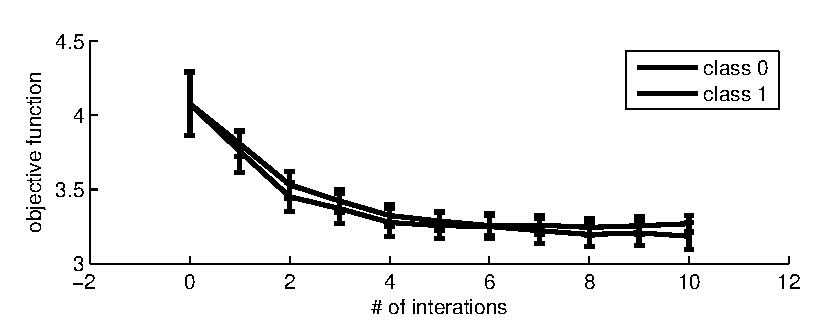
\includegraphics[width=.9\linewidth]{/Users/jovo/Research/figs/sims/unlabeled/homo_kidney_egg_obj}
\caption{objective function for simulation 1}
\label{fig:sim1_params}
\end{figure}


% subsubsection homogeneous_kidney_egg_simulations (end)



\subsubsection{heterogeneous simulations} % (fold)
\label{ssub:heterogeneous_simulations}

\begin{figure}[htbp]
	\centering		\includegraphics[width=1.0\linewidth]{/Users/jovo/Research/figs/sims/unlabeled/hetero_params}
	\caption{hetero model}
	\label{fig:models}
\end{figure}

\begin{figure}[htbp]
	\centering			\includegraphics[width=1.0\linewidth]{/Users/jovo/Research/figs/sims/unlabeled/hetero_Lhats}
	\caption{Lhats for hetero}
	\label{fig:figs_Sims_unlabeled_LPvsFW500}
\end{figure}


\begin{figure}[!ht]
\centering 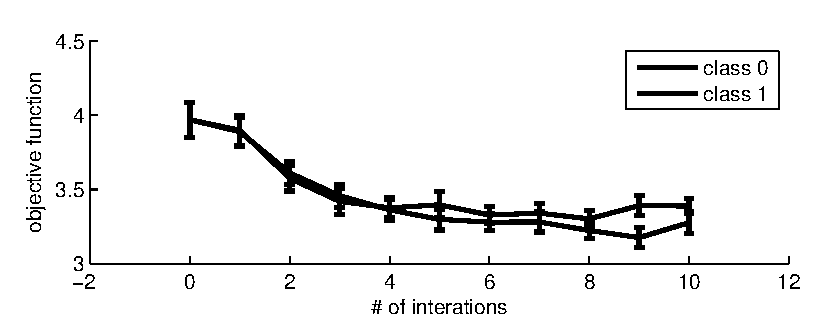
\includegraphics[width=.9\linewidth]{/Users/jovo/Research/figs/sims/unlabeled/hetero_obj}
\caption{objective function for hetero simulation}
\label{fig:sim1_params}
\end{figure}

% subsubsection heterogeneous_simulations (end)

% subsection simulation_results (end)

% subsection latent_permutation_matrix_approach (end)

% subsection graph_invariant_based_classifiers (end)

% section methods (end)


\subsection{C elegans simulations} % (fold)
\label{sub:c_elegans_simulations}


We took the C. elegans connectome, randomly permuted it, added noise, and then ran the same classification code with the following results....


% subsection c_elegans_simulations (end)

\clearpage
\section{Discussion} % (fold)
\label{sec:discussion}

XXX cep's original write-up had a bunch of stuff about signal subgraph finding.  it now seems quite unrelated to me.  perhaps we drop that bit? XXX

other graph matching approaches---inexact, get you closer

incorporating priors using distance

parallel implementations for large graphs


starting with ``truth'' or not

% section discussion (end)

\clearpage
\appendix

\section{Linear assignment problem solution} % (fold)
\label{ssub:linear_assignment_problem_solution}

% Solving \eqref{eq:a} is difficult for two reasons: (i) the objective function is not necessarily convex, and (ii) the constraints are nonlinear.  That the objective function is not necessarily convex is clear by virtue of computing the Hessian of the argument in \eqref{eq:a} with respect to $Q$:
% \begin{align}
% 	\nabla_Q^2 \mc{L} =  B \otimes A + B\T \otimes A\T,
% \end{align}
% where $\otimes$ indicates the Kronecker product, which is not positive definite (in general).  To resolve non-convexity, we can simply drop one of the $Q$'s from \eqref{eq:a}.  The implication of this is that instead of permuting both rows and columns, we only permute one or the other.  While this may seem like a totally ridiculous thing to do, crazier things have worked.  Given this simplification, the argument is not merely convex, but it is quadratic in $Q$, making solving it exactly feasible (independent of the constraints).  
% 
% To deal with the nonlinear of the constraints, we relax them to require that $Q$ merely be a doubly stochastic matrix.  A matrix is doubly stochastic if both its rows and columns sum to unity.  This is a ``natural'' relaxation in the sense that permutation matrices are doubly stochastic matrices, in fact, permutation matrices are the extreme points of the set of all doubly stochastic matrices, which we denote by $\mc{D}$.  

% Given the above two relaxations, we instead try to solve:
% \begin{align} \label{eq:a}
% 	\mh{Q} = \argmin_{Q \in \mc{D}} \norm{A Q\T - B}_F^2 = \argmin_{Q} \norm{A Q\T - B}_F^2 - \lambda (1 - \tfrac{1}{n}\mb{1}\T Q) - \lambda (1 - \tfrac{1}{n}\mb{1}\T Q\T),
% \end{align}
% where the second equality follows from replacing the linear constraint with its equivalent Lagrange multipliers.  If $\mh{Q}$ is not a permutation matrix, then projecting it onto its nearest permutation matrix is 
linear assignment problem:
\begin{align}
	\mh{Q}_{LAP} = \argmin_{Y \in \mc{Q}} \norm{\mh{Q} - Y}_F^2 = \argmin_{Y \in \mc{Q}} tr (Y\T \mh{Q})
\end{align}
which can be solved using the Hungarian algorithm in $\mc{O}(n^3)$, as shown in the below lemma. 

\begin{Lem}
  Given $Y \in \Real^{n \times n}$, the projection of $Y$ onto $\mc{Q}_n$ can
  be obtained by solving the linear assignment problem:
  $$ 
  \mh{W}= \argmin_{W \in \Pi_n} \norm{ W-Y}_F = \argmax_{W \in \mc{D}_n}  tr(YW\T)
  %   \Pi_n }\rbrace \equiv {\text{\rm arg }} \max_W \lbrace{ tr(YW^t)
  %   \mid W \in \mathcal D_n }\rbrace .
  $$
  Proof: Since $W \in \Pi_n \subset \mathcal O$, we have
  \begin{align}
  \norm{W-Y}_F^2 &= tr( (W-Y)\T (W-Y)) \\
  &= (\norm{Y}_F^2 + \norm{I}_F^2) - 2tr( Y W\T ). \qed
  \end{align}
\end{Lem}
where the trace rule follows from \cite{HornJohnson}.




% subsubsection bilinear_assignment_problem_solution (end)

% subsubsection linear_assignment_problem_solution (end)


\section{Preliminaries} % (fold)
\label{sec:preliminaries}



Consider $(G,Y),\{(G_i,Y_i)\}_{i=1}^s \overset{iid}{\sim} \PP_{GY}$,
with classes $Y:\Omega \rightarrow \{0,1\}$ and
(labeled) graphs $G:\Omega \rightarrow \mcG_n$,
where $\mcG_n$ denotes the collection of simple (labeled) graphs on $V=[n]$.

NB:
We consider simple graphs -- unweighted, undirected, with no loops,
so the adjacency matrices are binary, symmetric, and hollow;
our connectome applications
may involve {directed, loopy, weighted, attributed, multi} graphs \ldots
(And I use directed loopy graphs in my example Section \ref{Example} \dots
perhaps we should use directed loopy throughout? or undirected unloopy? what say you, John???)

The collection
$\mcT \equiv \{(G_i,Y_i)\}_{i=1}^s$ is the training sample
and $s$ is the training sample size;
$G$ is the graph to be classified,
and $Y$ is the true but unobserved class label.
For simplicity, we will assume that the prior probability of class membership
$\pi \equiv P[Y=1]$ is known to be $1/2$,
and the class-conditional sample sizes $S_y \equiv \sum_{i=1}^s I\{Y=y\}$
are fixed ($s_y$) rather than random variables ($S_y$)
with $s$ even and $s_0=s_1=s/2$.

We consider the independent edge model (IE),
so that for $y \in \{0,1\}$ the class-conditional distribution $F_{G|Y=y}$
is parameterized by a (symmetric, hollow)
$n \times n$ matrix $P_y$ with entries $p_{y;u,v} \in [0,1]$.

(NB: We will eventually *generalize* the independent edge model to RDPG \ldots and beyond!
But first, herein, we will *simplify* to independent edge block model (IEBM), for mathematical expediency.)

For this IE model, the Bayes optimal classifier for observed graph $G$
(equivalently, for observed (symmetric, hollow) $n \times n$ adjacency matrix $A=A(G)=[a_{u,v}]$)
is given by
\begin{eqnarray}
g^*(G) &=& \arg\max_y \prod_{(u,v) \in {V \choose 2}} f(a_{u,v};p_{y;u,v}),
\end{eqnarray}
where the Bernoulli probability $f(a;p)$ is given by
%$f(a;p) = p I\{a=1\} + (1-p) I\{a=0\}$.
$f(a;p) = p^{a} (1-p)^{1-a}$.

Alas, the graph $G$ is not observed;
rather, we observe the {\em unlabeled} version.
(right. we don't observe the class label.
but here i mean ``unlabeled'' in the ``assignment problem'' sense.
too.)
That is, rather than observing the adjacency matrix $A$,
we observe $\tildeA \equiv QAQ^T$ for some unknown permutation matrix $Q$.
\\
(NB: sorry John.  because of all the $P$s, i'm gonna use $Q$ for permutation matrices.  deal with it?)

% section preliminaries (end)



\section{An Assignment Problem Application}

%``assignment problem'' applications:
%(1) block assignment;
%(2) vertex assignment;
%(3) combination.

(This is Assignment Problem Application \#1.
E.g., voxels = vertices,
and voxels have been morphed to anatomical regions as per JV's description.
If we assume for \#1 that this region assignment is perfect,
we have the within-region vertex assignment problem.
This is this \dots
we disussed adding distance $d(u,u')$ and assuming that true assignment is more likely for smaller distances;
we discussed relaxing the perfect region assignment to $P[u \in$ correct region$]$;
we discussed other generalizations?)


%Let $d_{\hatP}(\tildeA,A_i) = ||\hatP \tildeA \hatP^T - A_i||_F.$
%Let $g_{NN}(G;P') = \arg\min_y \min_{i:Y_i=y} d_{P'}(\tildeA,A_i).$

%The {\em nearest assignment neighbor classifier} for
%the observed $\tildeA \equiv PAP^T$
%is given by
%$$g_{NAN}(G) = \arg\min_y \min_{i:Y_i=y} ||\hatP_i \tildeA \hatP_i^T - A_i||_F.$$
%
%If $P$ is known,
%then
%the nearest neighbor classifier
%$$g_{NN}(G) = \arg\min_y \min_{i:Y_i=y} ||P \tildeA P^T - A_i||_F$$
%satisfies
%$L(g_{NN}) \rightarrow L_{NN}(\PP_{GY}) \leq 2L^*$ [Cover \& Hart].
%
%Let us consider
%$$g(G) = \arg\min_y \min_{i:Y_i=y} \min_{\hatP} ||\hatP \tildeA \hatP^T - A_i||_{F(\mcE)}.$$

Consider the observed $\tildeA \equiv QAQ^T$.
For $i \in [s]$, let
\begin{eqnarray}\label{assignmenteqn}
\hatQ_i = \arg\min_{Q'} ||Q'^T \tildeA Q' - A_i||_F.
\end{eqnarray}
For each pair $(u,v)$, let $\sigma_i(u,v)$ be the reassignment through $Q$ and $\hatQ_i$.
That is, entries $a_{u,v}$ in $A$ are out of place due to unlabeledness in $\tildeA$,
and the assignment minimization attempts to put them back into place;
$\sigma_i(u,v)$ is the result of this attempt -- the assignment provided by
$\hatQ_i Q A Q^T \hatQ_i^T$.




\defa\label{nac}
The {\em naive assignment classifier} for the observed $\tildeA$ is given by
\begin{eqnarray}
g(G;\mcT) = {\arg\max_y \max_{i:Y_i=y} \prod_{(u,v) \in {V \choose 2}} f(a_{\sigma_i(u,v)};p_{y;u,v})}.
\end{eqnarray}
\defb

Note 1:
The classifier $g(G;\mcT)$ presented in Definition \ref{nac}
assumes that the class-conditional edge probabilities $p_{y;u,v}$ are known;
however, these probabilities are not used in the assignment equation \ref{assignmenteqn}.
(They could be? But they're not!)

Note 2:
We could employ a plug-in classifier,
using estimates in both the classifier and the assignment;
e.g., $\hatp_{y;u,v} = (s_y)^{-1} \sum_{i:Y_i=y} a_{i;u,v}$
and $\overline{A}_y = (s_y)^{-1} \sum_{i:Y_i=y} A_{i}$.
However, we would want to use {\em smoothed} estimates in the classifier
(to avoid degeneracy when $\hatp_{y;u,v}$ equals 0 or 1)
and {\em unsmoothed} estimates in the assignment.
This complicates the evaluation analysis;
we leave this more complicated (and more realistic) investigation for the future.

Note 3:
The classifier $g(G;\mcT)$ presented in Definition \ref{nac}
uses only the single probability-maximizing training assignment for each class.
This could be generalized either in the assignment (using $\overline{A}_y$)
or by processing the collection
$\{\prod_{(u,v) \in {V \choose 2}} f(a_{\sigma_i(u,v)};p_{y;u,v})\}_{i:Y_i=y}$
with methods more elaborate than the simple maximum.

Note 4:
We could also use nearest neighbor classifier \dots but i think this would be less tractable.

The advantage of the classifier $g(G;\mcT)$ presented in Definition \ref{nac}
is that the assignment methodology and only the assignment methodology is on trial!
Better classifiers could be considered,
but I'm trying to design a tractable investigation of assignment methodologies \dots

%\subsection{A Simpler Model: IEBM$(n,p,\mcE)$}

Under IE,
the difference between
$F_{G|Y=1}$ and $F_{G|Y=0}$
is wholly captured by the collection of marginal ``signal edges'' probabilities
$$\mcE \equiv \{(u,v) \in {V \choose 2}: p_{0;u,v} \neq p_{1;u,v}\}.$$
This collection $\mcE$ might be all of ${V \choose 2}$.
We hereby simplify IE to independent edge block model (IEBM), for mathematical expediency.
Let $\mcE = {V' \choose 2}$ for a collection $V'$ of $1 \leq m \leq n$ vertices,
and define
IEBM$(n,p,m)$ to be the model $\PP_{GY}$ defined by class-conditional probabilities
$p_{0;u,v}=p \neq 1/2$ and $p_{1;u,v}=1-p$ for all $(u,v) \in \mcE$
and $p_{0;u,v}=p_{1;u,v}=1/2$ for all $(u,v) \in {V \choose 2} \setminus \mcE$.
(In this case, all signal edges are created equally and all noise edges are created equally.)
Notice that
IEBM$(n,p,m)$ requires that $\mcE$ is a block --
the signal edges consist of precisely the potential interconnections between a set of $m$ vertices.
%so that $\mcE$ can be thought of as an $m \times m$ submatrix 


Let $s=2$ (one single training observation from each class).
%Assume (for evaluation purposes, but not for algorithm development)
%that $p_{0;u,v}=p \neq 1/2$ and $p_{1;u,v}=1-p$ for all $(u,v) \in \mcE \subset {V \choose 2}$
%and that $p_{0;u,v}=p_{1;u,v}=1/2$ for all $(u,v) \in {V \choose 2} \setminus \mcE$.
In this case, since all signal edges are created equally and all noise edges are created equally,
the performance of the classifier $g(G;\mcT)$
is monotonic in the number of signal edges recovered by $\sigma_1$ and $\sigma_2$.

%If the estimates $\hatp_{y;u,v}$ are consistent (converge to $\hatp_{y;u,v}$ as $s \rightarrow \infty$),
%then both of these classifiers are consistent (converge to Bayes optimal);
%that is, $L(g) \rightarrow L(g^*) \equiv L^*$,
%where 

Let the random variable $L(g) \equiv P[g(G;\mcT) \neq Y| \mcT]$
be the probability of misclassification for classifier $g$
conditioned on the training sample [see DGL 1996].
Under IEBM$(n,p,m)$ with $s=2$, we have that $L(g)$ depends on only $n,p,m$.
Define $L^* \equiv L(g^*)$.

\thma
For $\PP_{GY} \in$ IEBM$(n,p,m)$,
$L(g|T=t) < L(g|T=t-1)$ for all $t \in [2m-1]$,
where
\begin{eqnarray}
T_i \equiv |\{(u,v) \in \mcE: \sigma_i(u,v) \in \mcE\}|
\end{eqnarray}
and
$$T \equiv T_1 + T_2.$$
\thmb

Proof:
(Proof of this (alleged) monotonicity requires but a simple modification to Henry's proof?)

So, for this simple case,
we need concern ourselves with only the performance of the assignment algorithm in terms of $T_i$.

\thma
$T_1 =^{\mcL} T_2$ for this simple case.
\thmb

Proof:
(By construction? it's suppose to \dots that's why i set up the class-conditional edge probabilities
 $p_{y;u,v}$ to be reflective about $1/2$ in $y$.)




\section{Performance Degradation}

What is the performance degradation due to unlabeled-ness?

Case I:

\thma
$P[\hatQ_i = Q]=1$ for all $i$ implies $L(g)=L^*$.
\thmb

Proof:
If $P[\hatQ_i = Q]=1$ for all $i$
(that is, if the assignment algorithm gets the {\em right} answer --
not to be confused with the {\em best} answer
in terms of the optimization)
then $T_1=T_2=|\mcE|$ and hence $L(g)=L^*$.


Case II:

How about when the assignment algorithm gets the {\em best} answer
in terms of the optimization?
Perhaps we can work this out -- a theorem/proof?

\thma
$L_{n,p,\mcE}(g) =$ some *identifiable* function of $n,p,\mcE$?
\thmb

According to my calculations,
the only tricky bit is $I\{T_i(g_1,g_2) = t\}$
given two graphs $g_1,g_2 \in \mcG_n$.
That is, given two graphs (no randomness),
$T_i$ either equals $t$ or it doesn't
(after (arbitrarily?) accounting for non-uniqueness
of assignment solution $\hatQ$).
This looks like i could do it for $n=3$.
But then the combinatorics get silly.
BUT: maybe this is one of those things for which
generating function folks
could derive a {\em generating function} \dots?
at least for my simple stochastic block model
class-conditional distributions?


After Case I
(the assignment algorithm gets the {\em right} answer --
not to be confused with the {\em best} answer in terms of the optimization)
and Case II
(the assignment algorithm gets the {\em best} answer in terms of the optimization),
we will investigate approximation assignment algorithms based on the trade-off between
(1) computational complexity and
(2) classification performance
(either $L(g)$ directly, or in terms of the distribution of $T_i$).


The Monte Carlo example presented below (Section \ref{Example})
demonstrates significant but not complete performance degradation
due to a particular algorithm
({\bf lp.assign} in {\bf R} package {\bf lpSolve}).




\section{Example}\label{Example}

A Monte Carlo experiment (20000 paired replications) demonstrates that,
(using {\bf directed loopy} graphs for simplicity)
with $n=10, p=0.25$, and $|\mcE|=9$
(where $\mcE$ is in fact a $3 \times 3$ block)
the performance degradation due to the application of
{\bf lp.assign} in {\bf R} package {\bf lpSolve}
(with $Q=I$ specifying starting point)
is from
$\hatL = 0.0476 \approx L^* = 1-F_{Binomial(9,0.25)}(4) = 0.04892731\dots$
to
 $\hatL = 0.28855$.
So better-than-chance classification is achieved for our unlabeled scenario
using this assignment algorithm,
but performance is significantly degraded.

NB:
should also report performance in terms of $T_i$.
and objective value at solution?

Code for this example is provided in the Appendix.

NB: LAP is not QAP; i'd be happy to have QAP R code \dots

\section{Proposal}

I propose that we investigate,
via theory, simulation, and experiment,
the trade-off between computational complexity and performance,
and also identify the relationship between
the explicit assignment objective function
and the exploitation task (classification) objective function.

Except for Cases
I
(the assignment algorithm gets the {\em right} answer --
not to be confused with the {\em best} answer in terms of the optimization)
and
II
(the assignment algorithm gets the {\em best} answer in terms of the optimization),
I'm not sure what we'll be able to prove.
Perhaps
\thma
LAP is as good as QAP $\iff$ model $\in$ IEBM?
\thmb
But we can do simulation analysis:
first, for my simple scenaro;
then, generalizing to (perhaps) approach experimental settings?
\\

NB: perhaps we should be doing hypothesis testing instead???



\section{other} % (fold)
\label{sec:other}

% section other (end)


Finding the best alignment of vertices has been called the graph isomorphism problem (GIP) \cite{??}, and is known to be computationally equivalent to the quadratic alignment problem (QAP) \cite{??}.  Given to graphs, $A$ and $B$, the QAP can be formalized as follows:
\begin{align}
	\mh{P} = \argmin_{P \in \Pi} \norm{PAP\T - B}
\end{align}
where $\Pi$ is the set of all permutation matrices, that is, all matrices with a single one in each row and column, and zeros otherwise.  


We therefore investigate building classifiers on the space of collections of unlabeled graphs.  Specifically, we consider two distinct approaches. First, we build classifiers using ``graph invariants,'' that is, statistics of the graphs that are invariant to isomorphic translations.  Second, we first approximately solve the graph isomorphism problem,  



Data today are unlabeled graphs.  examples (mostly brain-graph examples)....

Previous work classifying unlabeled graphs..... Problem: consistency for what model?

Previous work classifying labeled graphs.... Problem: graph isomorphism

Previous work solving graph isomorphism problem.

Paper organization...


\section*{Appendix}

Code producing the example results presented in Section \ref{Example}.

\begin{verbatim}

library(lpSolve)
cuc = function(thisclass,myseed=1)
# Classification of Unlabeled Connectomes
{
set.seed(myseed)
n=10
nmc=10000
# directed, with loops
P1 = P2 = matrix(0.5,n,n) # class-conditional distribution specification
P1[1:3,1:3] = 0.25
P2[1:3,1:3] = 0.75
label = labeltilde = tie = tietilde = rep(0,nmc)
Qhat1lpobjval = Qhat2lpobjval = NULL
for(mc in 1:nmc)
{
G1 = matrix(rbinom(n^2,1,P1),n,n)
G2 = matrix(rbinom(n^2,1,P2),n,n)
if(thisclass == 1 )
 G  = matrix(rbinom(n^2,1,P1),n,n)
if(thisclass == 2 )
 G  = matrix(rbinom(n^2,1,P2),n,n)
Q = matrix(0,n,n)
diag(Q) = 1 # Q == I
Gtilde = Q %*% G %*% t(Q)
C1 = C2 = matrix(0,n,n) # cost
for(i in 1:n) for(j in 1:n)
 {
 C1[i,j] = sum(abs(Gtilde[i,]-G1[j,]))
 C2[i,j] = sum(abs(Gtilde[i,]-G2[j,]))
 }
Qhat1lp = lp.assign(C1)
Qhat2lp = lp.assign(C2)
Qhat1 = Qhat1lp$solution
Qhat2 = Qhat2lp$solution
Qhat1lpobjval[mc] = Qhat1lp$objval
Qhat2lpobjval[mc] = Qhat2lp$objval
sigma1 = t(Qhat1) %*% Gtilde
sigma2 = t(Qhat2) %*% Gtilde
# now ... classify G and Gtilde
p1 = prod( (P1^G) * ((1-P1)^(1-G)) )
p2 = prod( (P2^G) * ((1-P2)^(1-G)) )
p1tilde = prod( (P1^sigma1) * ((1-P1)^(1-sigma1)) )
p2tilde = prod( (P2^sigma2) * ((1-P2)^(1-sigma2)) )
if(p1>p2) label[mc]=1
if(p1==p2) tie[mc]=1
if(p1tilde>p2tilde) labeltilde[mc]=1
if(p1tilde==p2tilde) tietilde[mc]=1
}
return(list(label,tie,labeltilde,tietilde))
}

cuc1 = cuc(1)
cuc2 = cuc(2)

sum(cuc1[[1]])
sum(cuc1[[2]])
sum(cuc1[[3]])
sum(cuc1[[4]])
# [1] 9524
# [1] 0
# [1] 6986
# [1] 121

sum(cuc2[[1]])
sum(cuc2[[2]])
sum(cuc2[[3]])
sum(cuc2[[4]])
# [1] 476
# [1] 0
# [1] 2759
# [1] 117

(10000 - sum(cuc1[[3]]) - .5*sum(cuc1[[4]]) + sum(cuc2[[3]]) + .5*sum(cuc2[[4]]))/20000
# [1] 0.28855

# L*:
# > 1-pbinom(4,9,.25)
# [1] 0.04892731

\end{verbatim}

% \newpage

\subsection{move this \dots}

Under IE,
the difference between
$F_{G|Y=1}$ and $F_{G|Y=0}$
is wholly captured by the collection of marginal ``signal edges'' probabilities
$$\mcE \equiv \{(u,v) \in {V \choose 2}: p_{0;u,v} \neq p_{1;u,v}\}.$$
\begin{eqnarray}
g^*(G) &=& \arg\max_y \prod_{(u,v) \in {V \choose 2}} f(a_{u,v};p_{y;u,v}) \\
       &=& \arg\max_y \prod_{(u,v) \in \mcE} f(a_{u,v};p_{y;u,v}),
\end{eqnarray}

If we estimate $p_{y;u,v}$ from the training data,
we may consider classifiers
\begin{eqnarray}
g_{NB}(G;\mcT) = \arg\max_y \prod_{(u,v) \in {V \choose 2}} f(a_{u,v};\hatp_{y;u,v})
\end{eqnarray}
and
\begin{eqnarray}
g_{\mcE}(G;\mcT) = \arg\max_y \prod_{(u,v) \in \mcE} f(a_{u,v};\hatp_{y;u,v}).
\end{eqnarray}
NB: requires *smoothed* estimates $\hatp_{y;u,v}$,
to avoid degeneracy when $\hatp_{y;u,v}$ equals 0 or 1.

The latter classifier, $g_{\mcE}(G;\mcT)$,
is the best we can hope for -- it considers the signal edges and only the signal edges;
the former can be swamped by noise from non-signal edges.

If the estimates $\hatp_{y;u,v}$ are consistent (converge to $\hatp_{y;u,v}$ as $s \rightarrow \infty$),
then both of these classifiers are consistent (converge to Bayes optimal);
that is, $L(g) \rightarrow L(g^*) \equiv L^*$,
where the random variable $L(g) \equiv P[g(G) \neq Y| \{(G_i,Y_i)\}_{i=1}^s]$
is the probability of misclassification for classifier $g$
conditioned on the training sample [see DGL 1996].
Note that $g_{\mcE}(G;\mcT)$ should dominate $g_{NB}(G;\mcT)$.


% \paragraph{Acknowledgments}

% \appendix
\clearpage

\bibliography{/Users/joshyv/Research/latex/biblist}
\addcontentsline{toc}{section}{References}
%\bibliographystyle{apalike}
\bibliographystyle{ieeetr}
%\bibliographystyle{nature}



\end{document}